\section{Introduction}

\TODO{Recapitulate main points of project thesis:}

\TODO{some general intro about the possibility of quark stars}

In this chapter, we will study a hypothetical class of compact stars known as quark stars.
Let us summarize the main ingredients in this work.

\subsection{The Tolman-Oppenheimer-Volkoff equation}

In \cref{chap:tov} we derived the Tolman-Oppenheimer-Volkoff equation
\begin{subequations}
\begin{align}
	\odv{P}{r} &= -\frac{G m \epsilon(P)}{r^2 c^2} \left( 1 + \frac{P}{\epsilon(P)} \right) \left( 1 + \frac{4 \pi r^3 P}{m c^2} \right) \left( 1 - \frac{2 G m}{r c^2} \right)^{-1} , \\
	\odv{m}{r} &= \frac{4 \pi r^2 \epsilon(P)}{c^2} .
\end{align}
\end{subequations}
It determines the pressure and mass gradients with relativistic corrections inside a spherically symmetric star composed of a perfect fluid in hydrostatic equilibrium.
Given the fluid's equation of state $\epsilon(P)$ that relates its pressure $P$ to its energy density $\epsilon$, it is a system of two equations for the two unknowns $P$ and $m$ and can be integrated.
We will seek mass-radius solutions to the equation, obtained by integrating it from the center $r=0$ with zero initial mass $m(0) = 0$ and some central pressure $P(0) = P_c$ until reaching the surface $r=R$ defined by a vanishing pressure $P(R) = 0$ and where the mass $m(R) = M$ defines the star's total mass.
By finding such solutions for a range of central pressures $P_c$, we parametrize a sequence of stars that we can plot in a mass-radius diagram.

\subsection{Equation of state from thermal field theory}

To derive equations of state for quark matter, we will study quantum field theories whose dynamics is described by some Lagrangian density $\lagr$.
In \cref{chap:tft} we showed that the partition function in the grand canonical ensemble corresponding to a Lagrangian including both a fermionic field $\psi$ and a bosonic field $\phi$ is given by the path integral
\begin{equation}
	Z = \oint_- \pathintdif \bar{\psi} \oint_- \pathintdif \psi \oint_+ \pathintdif \phi \exp \Big\{ \int_0^\beta \dif \tau \int_V \dif^3 x \, \lagr_E[\bar{\psi}, \psi, \phi] \Big\} = e^{-\beta V \Omega} .
\end{equation}
Here $V$ is the spatial volume of the system, while its inverse temperature $\beta = 1/T$ define its ``temporal'' extent.
The sign subscripts on the closed integral signs is supposed to remind us of a property we showed extensively in \cref{chap:tft}: the bosonic fields must be periodic in inverse temperature time, while the fermionic fields must be anti-periodic.
If a symmetry of the Lagrangian admits a conserved Noether charge density $j^0$, we also saw that we could couple it to a chemical potential $\mu$ in the Lagrangian by including the term $\mu j^0$.
By computing (the logarithm of) the partition function, we have the grand potential $\Omega = -\log Z / \beta V$ from which we can calculate all thermodynamic quantities such as the (mean)
\TODO{this is already in $T=0$ form? write in general $T \geq 0$ form in this intro?}
\begin{equation}
	\text{density} \quad n = -\pdv{\Omega}{\mu}, \quad
	\text{pressure} \quad P = -\Omega, \quad
	\text{energy density} \quad \epsilon = -P + \sum_p \mu_p n_p .
\end{equation}
These expressions are valid in the approximation of zero temperature $T=0$ that we saw was valid for neutron stars in \cref{chap:nstars}.
As quark stars are expected to be ``more intense neutron stars'', we assume that this approximation still holds.

The equation of state $\epsilon(P)$ follows by eliminating the chemical potentials $\mu_p$ from the energy density $\epsilon(\mu_p)$ in favor of the pressure $P$.
In \cref{chap:nstars} we did so for pure neutron stars, for which there was only one chemical potential to eliminate.
Now we will study quark stars composed of up quarks, down quarks, strange quarks and electrons, each associated with their own chemical potential $\mu_p$.
With these \emph{four} particles, we require \emph{three} additional relations that reduce the dependence of the pressure and energy density to \emph{one} independent chemical potential, which can finally be eliminated to yield the equation of state.

\subsubsection{Chemical equilibrium of weak interaction processes}

We can obtain two relations between the chemical potentials by studying the nuclear processes that take place inside the star.
According to \cite{ref:quark_star_processes}, quarks stars may be formed as hadronic matter in a neutron star decays to strange quark matter through weak interactions processes like
\begin{equation}
	u + e^- \rightarrow d + \nu_e
	\qquad \text{and} \qquad
	u + e^- \rightarrow s + \nu_e .
\end{equation}
Over time, the star cools and neutrinos diffuse out. \cite[section 5.3]{ref:glendenning}
We therefore set $\mu_{\nu_e}=0$, so that the chemical equilibrium of the two processes above implies
\begin{equation}
	\mu_d = \mu_s = \mu_u + \mu_e .
\label{eq:lsm:chemical_equilibrium}
\end{equation}
These are the two announced relations between the four chemical potentials.

\subsubsection{Electric charge neutrality of stars}

The third and last additional relation relating the four chemical potentials is provided by electric charge neutrality.
We can make a strong and simple classical argument for why there can be no \emph{global} net electric charge in stars by comparing Newton's law of gravity and Coulomb's law.
Consider a test particle of mass $m$ and electric charge $q$ on the surface $R$ from the center of a star with total mass $M$ and electric charge $Q$.
In an idealized situation, the test particle is affected by the gravitational and electrostatic force, so that the total outwards radial force on it is
\begin{equation}
	F_\text{out} = -G \frac{M m}{R^2} + k_e \frac{Q q}{R^2} .
\end{equation}
Furthermore, suppose the star consists of a great number $N$ of particles weighing, each with mass $m < m_B$ that is lower than some heavy baryon mass $m_B$ and about one elementary charge $q \approx \pm e$.
We then have $M < N M_B$ and $m < m_B$.
If the star had an opposite charge $Q = \mp Z e$, then $F_\text{out} < 0$ and the test particle would stay in the star, seeking to neutralize it.
On the other hand, if the star has a like charge $Q = \pm Z e$, then
\begin{equation}
	F_\text{out} > -G \frac{N m_B^2}{R^2} + k_e \frac{Z e^2}{R^2} .
\end{equation}
Assuming a typical baryon mass $m_B = m_p = \SI{1.67e-27}{\kilogram}$,
we then surely have $F_\text{out} > 0$ provided that the number of elementary charges per particle satisfies
\begin{equation}
	\frac{Z}{N} > \frac{G m_B^2}{k_e e^2} \approx 10^{-37} .
\end{equation}
This means that particle are expelled from the star while $Z > 10^{-37} N$ until $Z$ has fallen to \emph{at least} $Z < 10^{-37} N$.
We conclude that for all practical purposes, stars are \emph{globally} electrically charge neutral.
As explained by \cite{ref:master_halvor}, this argument is slightly modified by relativistic corrections, but the conclusion is not.

In a star that consists of a set of particles $p$ each with charge $q_p$, we could implement \emph{global} charge neutrality by constraining the chemical potentials such that the charge density
\begin{equation}
	\sum_p q_p \, n_p(\mu_p) = \rho(r)
\label{eq:intro:charge_neutrality_global}
\end{equation}
at radius $r$ is equal to some charge density function $\rho(r)$ that causes the total charge $Q = \int \rho(r) 4 \pi r^2 \dif r = 0$ \TODO{add relativistic correction $e^{\beta(r)}$ from metric?} to vanish.
This approach would make the equation of state $\epsilon(P,r)$ dependent on radius in addition to pressure.
It is not obvious how one should single out one of the infinitely many possible charge density profiles $\rho(r)$.
We will avoid this problem altogether by rather assuming that charge neutrality holds \emph{locally} with $\rho(r) = 0$.
Then the equation of state $\epsilon(P)$ is again a function of pressure only, obtained by eliminating chemical potentials according to
\begin{equation}
	\sum_p q_p \, n_p(\mu_p) = 0
\label{eq:lsm:charge_neutrality}
\end{equation}
As shown in \cite{ref:global_neutrality}, for example, this simplification can modify the masses and radii of stars within an order of magnitude, but the differences are smaller closer to the maximum mass star.
In fact, \cite{ref:local_neutrality_inconsistent} has shown that local charge neutrality in neutron stars composed of protons, neutrons and electrons is unphysical.
Our choice $\rho(r)=0$ is therefore the simplest choice, but not the most physical one.

\section{Color confinement, asymptotic freedom and bag models}

(Inspired by \cite{ref:quark_bag_model})

\TODO{discuss $\epsilon$, $P$ before this}
\TODO{understand bag-constant as a measure of the trace anomaly? $m = 0$ -- conformal inveriance, classical symmetry broken in the quantum case?}
\TODO{justify and make less ad-hoc, move some of this to intro?}
\TODO{understand difference between $P(\mu)$ and $P(\mu,B)$}
\TODO{find source on bag stuff. JO?}
\TODO{difference between ``perturbative vacuum'' and ``confined vacuum''}

\begin{figure}
\centering
\tikzsetnextfilename{bag-model}
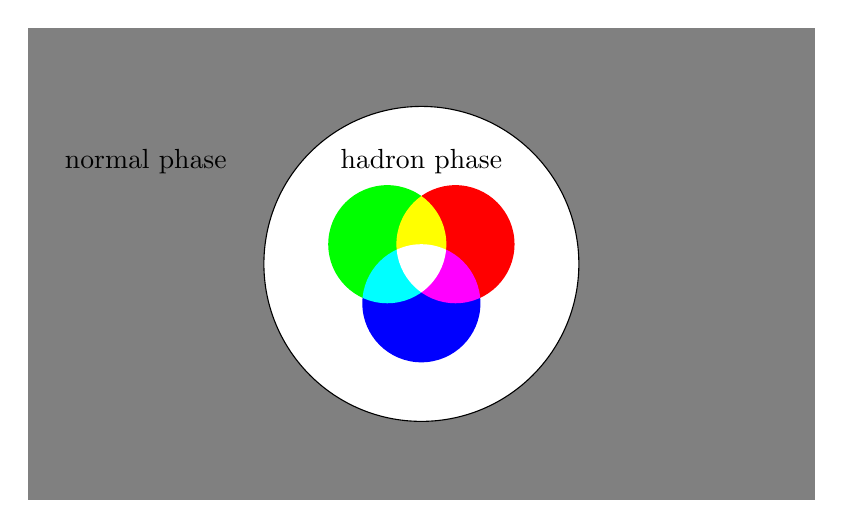
\begin{tikzpicture}
\fill [gray] (-5, -3) rectangle (+5, +3);

\draw [draw=black, fill=white] (0, 0) circle (2);
\begin{scope}[blend group=screen]
	\fill [fill=red]   (30:0.5)  circle (0.75) node {$u$};
	\fill [fill=green] (150:0.5) circle (0.75) node {$d$};
	\fill [fill=blue]  (270:0.5) circle (0.75) node {$s$};
\end{scope}
\node at (90:1.3) {hadron phase};
\node at (-3.5,1.3) {normal phase};
\end{tikzpicture}
\caption{\label{fig:lsm:confinement}%
	\TODO{caption}
}
\end{figure}

\textbf{Color confinement} is a fundamental feature of quantum chromodynamics.
Experiments and lattice simulations have shown that color-charged particles like quarks cannot be isolated from each other, but are rather confined in hadrons.
Quarks can be color-charged \textcolor{red}{\textbf{red}}, \textcolor{green}{\textbf{green}} and \textcolor{blue}{\textbf{blue}},
while antiquarks can have the complementary colors -- or anticolors -- \textcolor{cyan}{\textbf{antired}}, \textcolor{magenta}{\textbf{antigreen}} and \textcolor{yellow}{\textbf{antiblue}}.
For example, a meson consists of one quark of any color and one antiquark with the complementary color of the first quark, making the meson itself \emph{colorless}.
Similarly, a baryon consists of one red, one green and one blue quark,
while an antibaryon consists of one antired, one antigreen and one antiblue quark,
and are thus also colorless.

Another important property of quantum chromodynamics is \textbf{asymptotic freedom}.
As the energy scale of quark interactions increases -- or its length scale decreases -- the \emph{strength} of the interactions \emph{decreases}!
Consequently, 
This property was first discovered by \cite{ref:asymptotic_freedom_gross_wilczek,ref:asymptotic_freedom_politzer} and recognized with the Nobel Prize in 2004.

Together, these two features explain that at high temperature or high density,
quarks become \emph{deconfined} in the sense that they are free of interactions between each other,
but their positions are spatially \emph{confined} to a hadron.
In an extremely dense pure neutron star, for example,
the neutrons' three constituent quarks would break free from each other and hence the bound neutron state due to asymptotic freedom,
but would still be spatially confined to the extent of the original neutron because of color confinement.

To model quark matter and the effect of these two properties,
physicists have come up with various \textbf{bag models}.
As illustrated in \cref{fig:lsm:confinement}, these models split the medium of the physical vacuum state into two phases.
The \emph{normal phase} is the background phase in which quarks are forbidden to exist -- remains of the non-confining medium that existed before the separation into two phases.
On top of the background, bubbles of \emph{hadron phase} are created inside which colorless combinations of quarks are confined.
Mathematically, the confinement is implemented by adding a bag constant $B$ to the grand potential density $\Omega$ of the quarks assumed to live inside the hadronic bubbles.
The bag constant is therefore defined as the energy difference between the hadronic phase and the normal phase,
and creating a hadronic bubble of volume $V$ costs the energy $B V$.
A positive bag constant gives a negative contribution to the pressure $P = -\Omega$,
hence confining the contents of the bag with an external pressure from the surrounding medium in the normal phase.

The \textbf{MIT bag model} is the simplest example.
Consider a star composed of up, down and strange quarks in the zero-temperature and massless approximation.
According to what we learned in \TODO{ref 4.12} and \eqref{eq:nstars:ur_eos}, the grand potential ``before bagging'' is
Pressure
\begin{equation}
	P(\mu) = \smashoperator{\sum_{f=\{u,d,s\}}} \frac{N_c \mu_f^4}{12 \pi^2}
	\qquad \text{and} \qquad
	\epsilon(\mu) = -P(\mu) + \smashoperator{\sum_{f=\{u,d,s\}}} \frac{N_c \mu_f^4}{3 \pi^2}.
\end{equation}
After ``bagging'' the quarks with a bag constant $B$,
\begin{equation}
\begin{split}
	P(\mu,B) = P(\mu) - B, \\
	\epsilon(\mu,B) = -P(\mu,B) + \smashoperator{\sum_{f=\{u,d,s\}}} \frac{N_c \mu_f^4}{3 \pi^2}.
	                = -P(\mu,B) + 4 (P(\mu,B) + B) = 4 P(\mu,B) + 4 B.
\end{split}
\end{equation}
The energy density and equation of state is then
\begin{equation}
	\epsilon(P) = -P + \sum_f \mu_f n_f = -P + \sum_f \frac{N_c \mu_f^4}{3 \pi^2} = -P + 4P = 3P
\end{equation}
To ``bag'' the quarks, the idea is 

In the early days of high density and temperature, the universe likely passed through a deconfined quark matter phase.
Today, matter is accreting by nuclear fusion in stars towards iron-56, seemingly representing the ground state of nuclear matter.
However, \cite{ref:strange_hypothesis_bodmer} and \cite{ref:strange_hypothesis_witten} has hypothesized that this state of matter is only \emph{metastable}.
Their \textbf{strange matter hypothesis} claims that the true ground state of nuclear matter is that of three-flavor matter consisting of up, down and strange quarks

\TODO{rewrite?}
We can use the presumed stability of two-flavor and three-flavor quark matter to determine a range of acceptable windows for the bag constant $B$.
Per baryon, iron-56 has an energy of $E/N_B = \epsilon/n_B = \SI{930}{\mega\electronvolt}$,
so if $\epsilon_2$ and $\epsilon_3$ are the energy densities of two-flavor and three-flavor quark matter,
we determine the bag constant $B$ such that
\TODO{at zero pressure?}
\begin{equation}
	\frac{\epsilon_3(0)}{n_B} < \SI{930}{\mega\electronvolt} < \frac{\epsilon_2(0)}{n_B} .
\label{eq:lsm:bag_stability}
\end{equation}
Only the two-flavor bound has been observed,
while the three-flavor bound is a quite reckless assumption that should certainly be taken with a grain of salt.
It will, however, be very useful to have \emph{some} bound for the bag constant in order to constrain the parameter space of equations of state later on.

\TODO{titles}

\TODO{units, $\hbar = c = G = k_B = 1$ or not?}

\TODO{organize project and master thesis together}

\section{Quantum chromodynamics and effective field theory}

\TODO{philosophy of effective field theory: identifty DoF (particles) and symmetries, write down most general Lagrangian with all (relevant) interactions \cite{ref:weinberg_eft}. like small oscillations in classical mechanics?}

\TODO{what about radius $r < R$ instead of $r=R$?}

\TODO{what about general relativity instead of Newtonian gravity?}

\TODO{what about contribution from pressure and other things to $F_\text{out}$?}

\TODO{can I recast inequality in charge per solar mass? see discussion at beginning of \url{www.if.ufrgs.br/hadrons/MMalheiro.pdf}}


\subsection{Symmetries}

Always have $U(1)_V$ symmetry, giving rise to conservation of baryon number.

Symmetry breaking
\begin{equation}
	SU(2)_L \times SU(2)_R \quad \rightarrow \quad SU(2)_V
\end{equation}
Quark-meson model can be written in terms of left/right fields:
\begin{equation}
\begin{split}
	\bar{\psi} \phi_5 \psi &= \bar{\psi} ( (P_+ + P_-) \sigma + (P_+ - P_-) i \tau \cdot \pi) \psi \\
	                       &= \bar{\psi} ( P_+ (\sigma + i \tau \cdot \pi) + P_- (\sigma - i \tau \cdot \pi) ) \psi \\
	                       &= \bar{\psi} ( P_+ \phi + P_- \phi^\dagger) \psi \\
	                       &= \bar{\psi} ( P_+ \phi P_+ + P_- \phi^\dagger P_-) \psi \\
	                       &= \bar{\psi}_- \phi P_+ + \bar{\psi}_+ \phi^\dagger \psi_- \\
\end{split}
\end{equation}
Used that $P_\pm^2 = P_\pm$ is in spinor-space, while $\phi$ is in flavor space.
Denote $+ = R$, $- = L$.
Now it is apparent that LSM is invariant under $SU(2)_L \times SU(2)_R$:
\begin{equation}
	\psi_+ \rightarrow U_+ \psi_+, \qquad
	\psi_- \rightarrow U_- \psi_-, \qquad
	\phi   \rightarrow U_- \phi U_+^\dagger.
\end{equation}
When $h \neq 0$, this symmetry is explicitly broken.



